\appendix
\chapter{Esercizi Svolti}

\textbf{Codifica di sorgente}

\begin{enumerate}
 \item Determinare se il codice con le seguenti parole è univocamente decodificabile o meno: 
       012, 0123, 4, 310, 1024, 2402, 2401, 4013.
       \bigskip
       \bigskip

       \textit{Soluzione:}

       \noindent
       Si può utilizzare l'algoritmo di Sardinas-Patterson. Risulta:
       \begin{table}[htbp]
       \begin{center}
       \begin{tabular}{l | l | l | l | l | l | l | l | l | l | l | l}
        $S_0$ & $S_1$  & $S_2$ & $S_3$ & $S_4$ & $S_5$ & $S_6$ & $S_7$ & $S_8$ & $S_9$ & $S_{10}$\\
        \hline
        012  & 3   & 10 & 24 & 02 & 2  & 402 & 3  & 10 & 24  & 3 \\
        0123 & 013 &    &    & 01 & 23 & 401 & 01 & 2  & 402 & 01 \\
        4    &     &    &    &    &    &     & 02 & 23 & 401 & 02 \\
        310  &     &    &    &    &    &     &    &    &    & \\
        1024 &     &    &    &    &    &     &    &    &    & \\
        2402 &     &    &    &    &    &     &    &    &    & \\
        2401 &     &    &    &    &    &     &    &    &    & \\
        4013 &     &    &    &    &    &     &    &    &    & \\
       \end{tabular}
       \end{center}
       \end{table}

       Il codice è dunque UD, poiché $S_{10}$ coincide con $S_7$.

       \bigskip
 \item Si costruisca un codice di Shannon binario, per la seguente varabile aleatoria:
       \[ X = \left(
        \begin{array}{cccccccc}
           x_1  & x_2  & x_3  & x_4  & x_5  & x_6  & x_7  & x_8 \\
           0.22 & 0.02 & 0.20 & 0.18 & 0.05 & 0.08 & 0.15 & 0.10 \\
        \end{array} \right)
       \]
       Si stabilisca se la lunghezza media del codice ottenuto coincide con l'entropia di X (in base 2) senza calcolare 
       né l'una né l'altra.
       \bigskip
       \bigskip

       \textit{Soluzione:}

       \noindent
       Calcoliamo le lunghezze delle varie parole di codice, per il codice di Shannon. Deve essere:
       \[
        l_i=\left \lceil -log p_i \right \rceil
       \]
       Le lunghezze sono dunque:
       \[ L = \left(
        \begin{array}{cccccccc}
           x_1  & x_2  & x_3  & x_4  & x_5  & x_6  & x_7  & x_8 \\
           3    & 6    & 3    & 3    & 5    & 4    & 3    & 4 \\
        \end{array} \right)
       \]
       Un codice con queste lunghezze è ad esempio:
       \[ C = \left(
        \begin{array}{cl}
           x_1  & \to 000 \\
           x_2  & \to 111111 \\
           x_3  & \to 011 \\
           x_4  & \to 100 \\
           x_5  & \to 11000 \\
           x_6  & \to 0101 \\
           x_7  & \to 001  \\
           x_8  & \to 1101 \\
        \end{array} \right)
       \]

       Per il teorema \ref{limitelcodice}, la lunghezza media del codice coincide con l'entropia se e solo se:
       \[
        \forall i=1..n  \ \ p_i=D^{-l_i}
       \]
       Ma non è questo il caso (ad esempio $0.22\ne2^{-3}$). La lunghezza del codice non coincide quindi con 
       l'entropia di X.
       \bigskip

 \item Si determini se i seguenti codici sono univocamente decodificabili o meno:
       \begin{itemize}
        \item $C_1=\{10,010,1,1110\}$
        \item $C_2=\{0,001,101,11\}$
        \item $C_3=\{0,2,03,011,104,341,11234\}$
       \end{itemize}
       \bigskip
       \bigskip

       \textit{Soluzione:}

       \noindent
       Si può utilizzare l'algoritmo di Sardinas-Patterson. Risulta:
       \newpage

       \begin{table}[htbp]
       \begin{center}
       \begin{tabular}{l | l | l}
        $S_0$ & $S_1$  & $S_2$ \\
        \hline
        10   & 0   & 10  \\
        010  & 110 &     \\
        1    &     &     \\
        1110 &     &     \\
       \end{tabular}
       \end{center}
       \end{table}

       Quindi $C_1$ non è UD, poiché $S_0 \cap S_2 = \{10\} \neq \varnothing $.

       \begin{table}[htbp]
       \begin{center}
       \begin{tabular}{l | l | l | l | l}
        $S_0$ & $S_1$  & $S_2$ & $S_3$ & $S_4$\\
        \hline
        0   & 01 & 1 & 1  & 1  \\
        001 &    &   & 01 & 01 \\
        101 &    &   &    &    \\
        11  &    &   &    &   \\
       \end{tabular}
       \end{center}
       \end{table}

       Quindi $C_2$ è UD, in quanto $S_3=S_4$.

       \begin{table}[htbp]
       \begin{center}
       \begin{tabular}{l | l | l | l | l | l | l | l}
        $S_0$ & $S_1$  & $S_2$ & $S_3$ & $S_4$ & $S_5$ & $S_6$ & $S_7$ \\
        \hline
        0     & 3  & 41  & 34 & 1 & 04   & 4 &\\
        2     & 11 & 234 &    &   & 1234 &   &\\
        03    &    &     &    &   &      &   &\\
        011   &    &     &    &   &      &   &\\
        104   &    &     &    &   &      &   &\\
        341   &    &     &    &   &      &   &\\
        11234 &    &     &    &   &      &   &\\
       \end{tabular}
       \end{center}
       \end{table}

       Quindi $C_3$ è UD perché $S_7=\varnothing$.

        \bigskip
\item Si costruisca un codice ottimale ternario per la seguente variabile aleatoria:
      \[ X = \left(
        \begin{array}{cccccccc}
           x_1  & x_2  & x_3  & x_4  & x_5  & x_6  & x_7  & x_8 \\
           0.22 & 0.02 & 0.20 & 0.18 & 0.05 & 0.08 & 0.15 & 0.10 \\
        \end{array} \right)
       \]
       Si stabilisca se la lunghezza media del codice ottenuto coincide con l'entropia di X (in base tre) 
       senza calcolare né l'una né l'altra.
       \bigskip
       \bigskip

       \textit{Soluzione:}

       \noindent
       Si può utilizzare l'algoritmo di Huffman. Poiché è richiesto un codice ternario, deve essere n=1 mod 2.
       E' necessario quindi aggiungere un simbolo aggiuntivo (infatti 9=4*2+1).
       Risulta:
       \begin{table}[htbp]
       \begin{center}
        \begin{tabular}{l || l|l|| l|l|| l|l|| l|l}
            &$S_0$ &$C_0$&$S_1$       & $C_1$& $S_2$        & $C_2$& $S_3$        & $C_3$ \\
       \hline
      $x_1$ & 0.22 &2  & 0.22           &2  &$\boxed{0.25}$ & 1  &$\boxed{0.53}$  & 0 \\
      $x_3$ & 0.20 &00 & 0.20           &00 &0.22           & 2  &0.25            & 1 \\
      $x_4$ & 0.18 &01 & 0.18           &01 &0.20           & 00 &0.22            & 2 \\
      $x_7$ & 0.15 &02 & 0.15           &02 &0.18           & 01 &                & \\
      $x_8$ & 0.10 &10 & 0.10           &10 &0.15           & 02 &                & \\
      $x_6$ & 0.08 &11 & 0.08           &11 &               &    &                & \\
      $x_5$ & 0.05 &120 & $\boxed{0.07}$ &12 &               &    &                & \\
      $x_2$ & 0.02 &121 &                &   &               &    &                & \\
        \hline
            & 0    &122 & & & & & &\\    
       \end{tabular}
       \end{center}
       \end{table} 

      \noindent
      Un codice ottimale è dunque:
       \[ C = \left(
        \begin{array}{cl}
           x_1  & \to 2 \\
           x_2  & \to 121 \\
           x_3  & \to 00 \\
           x_4  & \to 01 \\
           x_5  & \to 120 \\
           x_6  & \to 11 \\
           x_7  & \to 02  \\
           x_8  & \to 10 \\
        \end{array} \right)
       \]

       La lunghezza del codice non coincide con l'entropia, perché X non è 3-adica. Infatti, ad esempio, 
       $-log_3 0.22 \simeq 1.37 \neq 1 $
        \bigskip
\item E' possibile costruire un codice binario univocamente decodificabile con lunghezze di parola 2,2,3,3,3,4,4,4? 
      Giustificare la risposta.
       \bigskip
       \bigskip

       \textit{Soluzione:}

       \noindent
       E' sufficiente utilizzare la diseguaglianza di McMillan. Risulta:
       \[
        2^{-2}+2^{-2}+2^{-3}+2^{-3}+2^{-3}+2^{-4}+2^{-4}+2^{-4}=1.0625>1
       \]
       Quindi non è possibile costruire un codice UD con queste lunghezze.

       \bigskip
\item Si stabilisca se la seguente affermazione è vera o falsa: ``Sia C un codice si sorgente binario con lunghezze 
di parola $l_1,l_2,...,l_n$. Se :
\[
 \sum_{i=1}^n 2^{-l_i} \le 1
\]
allora C è istantaneo''. Nel primo casi si fornisca una dimostrazione, nel secondo un controesempio.
\bigskip
       \bigskip

       \textit{Soluzione:}

       \noindent
       L'affermazione è falsa. La disuguaglianza di Kraft (\ref{kraft}) alla quale si fa riferimento,
        parla infatti di condizione 
       \textbf{affinchè sia possibile} costruire un codice istantaneo. Un controesempio può essere il seguente:
       \[ C = \left(
        \begin{array}{cl}
           x_1  & \to 00 \\
           x_2  & \to 0 \\
        \end{array} \right)
       \]
       Il codice rispetta la disuguaglianza, infatti:
       \[
        2^{-2}+2^{-1}=0.75<1
       \]
       Tuttavia si nota immediatamente che il codice non è istantaneo.

       \bigskip

\item Si costruisca un codice binario ottimale per la seguente variabile aleatoria:
      \[ X = \left(
        \begin{array}{cccccccc}
           x_1  & x_2  & x_3  & x_4  & x_5  & x_6  & x_7\\
           0.49  & 0.26 & 0.12 & 0.04 & 0.04 & 0.03 & 0.02 \\
        \end{array} \right)
       \]
Calcolare l'entropia di X e confrontarla con la lunghezza media del codice costruito.
       \bigskip
       \bigskip

       \textit{Soluzione:}

       \noindent
       Si può utilizzare l'algoritmo di Huffman.
       Risulta:
       \begin{table}[htbp]
       \begin{center}
        \begin{tabular}{l || l|l|| l|l|| l|l|| l|l|| l|l|| l|l}
     &$S_0$ &$C_0$&$S_1$       & $C_1$& $S_2$        & $C_2$& $S_3$  & $C_3$& $S_4$      &$C_4$ & $S_5$ & $C_5$    \\
       \hline
$x_1$& 0.49&1   & 0.49          &1   &0.49          &1  &0.49          &1 &0.49          &1 &$\boxed{0.51}$& 0\\
$x_2$& 0.26&00  & 0.26          &00  &0.26          &00 &0.26          &00&0.26          &00&0.49 & 1\\
$x_3$& 0.12&011 & 0.12          &011 &0.12          &011&$\boxed{0.13}$&010&$\boxed{0.25}$&01&     &\\
$x_4$& 0.04&01000& $\boxed{0.05}$&0101&$\boxed{0.08}$&0100&0.12          &011& & & &\\
$x_5$& 0.04&01001& 0.04          &01000&0.05          &0101&              &  & & & &\\
$x_6$& 0.03&01010& 0.04          &01001&              &    &              &  & & & &\\
$x_7$& 0.02&01011&               &    &              &    &              &  & & & &\\
       \end{tabular}
       \end{center}
       \end{table} 

      Un codice ottimale è dunque:
       \[ C = \left(
        \begin{array}{cl}
           x_1  & \to 1 \\
           x_2  & \to 00 \\
           x_3  & \to 011 \\
           x_4  & \to 01000 \\
           x_5  & \to 01001 \\
           x_6  & \to 01010 \\
           x_7  & \to 01011  \\
        \end{array} \right)
       \]

Calcoliamo ora l'entropia della variabile X:
\[
 H(X)=-\sum_{i=1}^7 p_i log(p_i) \simeq 2.013
\]
E la lunghezza del codice:
\[
 L(C)=\sum_{i=1}^7 p_i l_i =2.02
\]
Quindi $H(X)<L(C)$, ed infatti X non è 2-adica.
\bigskip
\end{enumerate}


\textbf{Capacità di canale}

\begin{enumerate}
 \item Si costruisca un canale ponendo in cascata due BSC con probabilità di errore $p_1$ e $p_2$, rispettivamente.
       Si determini la sua matrice di canale e se ne calcoli la capacità.
       \bigskip
       \bigskip

       \textit{Soluzione:}

       \noindent
       La matrice del canale è data dal prodotto dei due BSC, quindi:
      \[
       P = \left[
         \begin{array}{cc}
         (1-p_1)(1-p_2) + p_1 p_2 & (1-p_1)p_2 + p_1(1-p_2) \\
         p_1 (1-p_2)+(1-p_1)p_2 & p_1 p_2 +(1-p_1)(1-p_2)\\
         \end{array} \right]
      \]
      Semplificando:
      \[
       P = \left[
         \begin{array}{cc}
         1-(p_1+p_2-2p_1p_2) & p_1+p_2-2p_1p_2 \\
         p_1+p_2-2p_1p_2 & 1-(p_1+p_2-2p_1p_2)\\
         \end{array} \right]
      \]
      Si ottiene dunque ancora un BSC, in cui $p=p_1+p_2+2p_1p_2$.
      Poiché la capacità di un BSC è 1-H(p), si ottiene:
      \[
       C=1-H(p_1+p_2+2p_1p_2,1-[p_1+p_2+2p_1p_2])
      \]
      \bigskip

 \item Un canale discreto senza memoria è alimentato da una sorgente binaria $X \in \{0,1\}$ e produce in uscita 
       Y=X+Z, dove Z è una variabile aleatora indipendente da X, a valori nell'insieme $\{0,a\}$ e con distribuzione 
       di probabilità uniforme: $P\{Z=0\}=P\{Z=a\}=\frac{1}{2}$. Si calcoli la capacità di questo canale.
       Si noti che l'alfabeto di uscita del canale e la sua capacità dipendono dal valore di a.
       \bigskip
       \bigskip

       \textit{Soluzione:}

       \noindent
       Il grafo di canale è rappresentato in figura \ref{fig:gres}.

       \begin{figure}[htbp]
       \begin{center}
	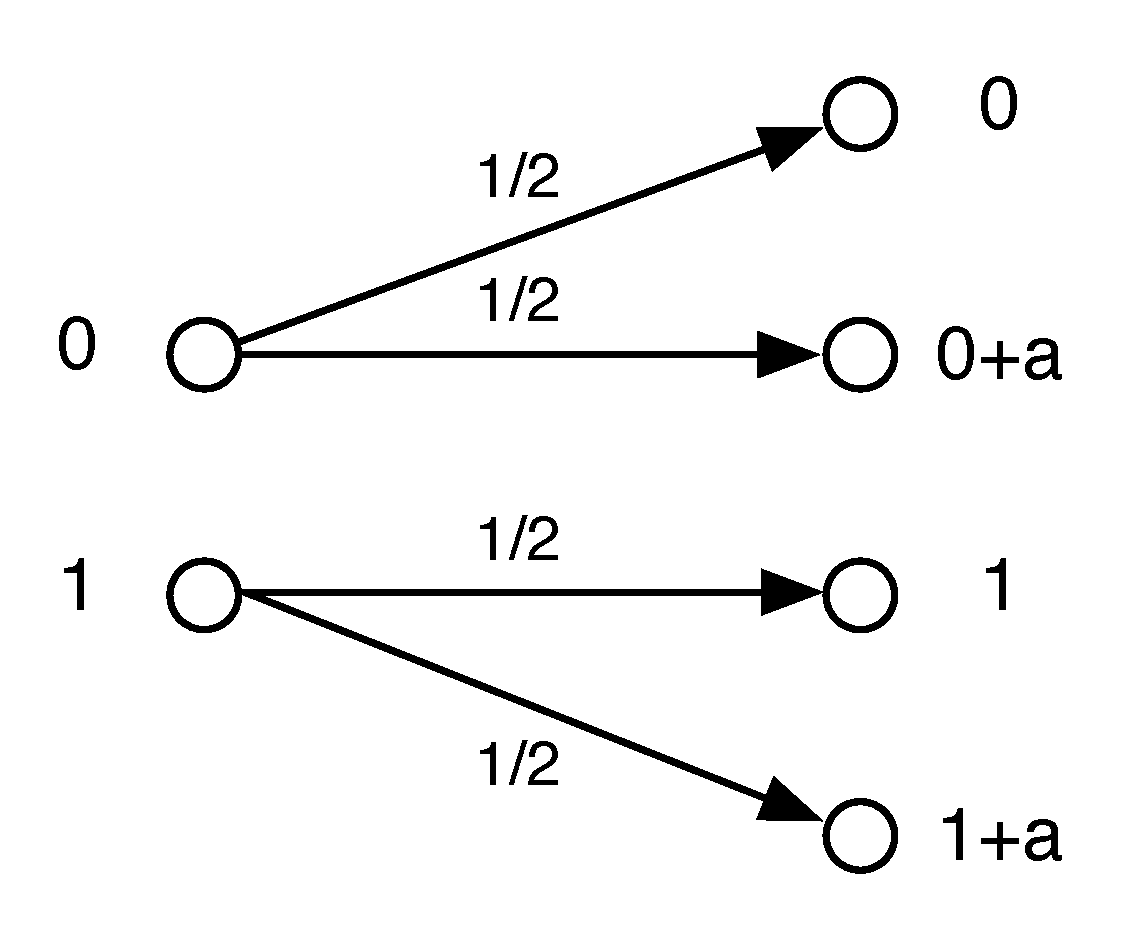
\includegraphics[width=0.4\textwidth]{img/gres.pdf}
       \caption{Grafo di canale}
       \label{fig:gres}
       \end{center}
       \end{figure}

       Poniamoci inizialmente nel caso in cui $a \neq 0$ e $a \neq 1$.
       Indicando con $\Pi$ $Pr\{X=0\}$, si ottiene:
       \[\begin{split}
        Pr\{Y=0\} &=\frac{\Pi}{2}  \\
        Pr\{Y=a\} &=\frac{\Pi}{2}  \\
        Pr\{Y=1\} &=\frac{1-\Pi}{2}  \\
        Pr\{Y=1+a\} &=\frac{1-\Pi}{2}  \\
        \end{split}
       \]
       Inoltre:
       \[
        H(Y/X=0)=H(Y/X=1)=H \left( \frac{1}{2},\frac{1}{2} \right)=1
       \]
       Quindi:
       \[\begin{split}
         I(X;Y) &=H(Y)-H(Y/X) \\
          &=H(Y)-\Pi H(Y/X=0) - (1-\Pi) H(Y/X=1) \\
          &=H(Y)-\Pi -1 + \Pi \\
          &=H(Y)-1 \\
          &=H \left (\frac{\Pi}{2},\frac{\Pi}{2},\frac{1-\Pi}{2},\frac{1-\Pi}{2} \right)-1 \\
         \end{split}
       \]
       Quindi la capacità è:
       \[
        C=\max_{p(x)} I(X;Y)
         =\max_{p(x)}H \left (\frac{\Pi}{2},\frac{\Pi}{2},\frac{1-\Pi}{2},\frac{1-\Pi}{2} \right)-1
       \]
       Ma il massimo dell'entropia si ha quando tutte le componenti sono uguali.
       In questo caso quindi si ha massimo quando valgono tutte 1/4, caso che si verifica per $\Pi=1/2$ (l'entropia 
       risulta invece log4=2).
       Risulta quindi:
       \[
        C=2-1=1 \ bit
       \]
       Restano da trattate i casi con a=0 e a=1. Se a=0, Y vale unicamente 0 o 1. Si ottiene un canale completamente 
       deterministico, la cui capacità è $C=log|X|=1$. Nel caso invece in cui a=1, Y assume i valori 0,1,2.
       In questo caso si ha un canale inutile, quindi la capacità è 0.
       Riassumendo:
       \[
        C=
        \begin{cases}
         1 & a \neq 1 \\
         0 & a =1 \\
         \end{cases}
        \]


       \bigskip
 \item Si calcoli la capacità del canale avente la seguente matrice di transizione:
      \[ P = \left(
        \begin{array}{ccccc}
           0.3  & 0.1  & 0.2 & 0.1 & 0.3 \\
           0.1  & 0.3  & 0.2 & 0.3 & 0.1\\
        \end{array} \right)
       \]
       e determinare una distribuzione di probabilità di ingresso in corrispondenza della quale si ottiene la capacità.
       \bigskip
       \bigskip

       \textit{Soluzione:}

       \noindent
       Si tratta di un canale debolmente simmetrico, pertanto:
       \[\begin{split}
        C &= log|Y|-H(r) \\
          &= log(5) - H(0.3,0.1,0.2,0.1,0.3) \\
          &\simeq 2.322 - 2.171 \\
          &\simeq 0.151 \ bit
         \end{split}
       \]
       La capacità si ottiene, sempre in virtù del fatto che il canale è debolmente simmetrico, quanto P(X) ha 
       distribuzione uniforme: X=(1/2,1/2).

       \bigskip
 \item In un canale binario, la probabilità che durante la trasmissione un bit venga complementato 
       (cioè, che da 0 diventi 1 e viceversa) è costante e pari a p=0.1.
        Assumendo che la sorgente che alimenta il canale invii un simbolo ogni secondo, è possibile 
        trasmettere informazione affidabile su questo canale ad una velocità superiore a 1 bit/sec. Perché?
       \bigskip
       \bigskip

       \textit{Soluzione:}

       \noindent
       Si tratta di un BSC, la cui capacità è:
       \[
        C=1-H(p)=1-H(0.1,0.9) \simeq 1-0.469 \simeq \ 0.531 bit
       \]
       Per il secondo teorema di Shannon, per trasmettere informazione affidabile deve essere :
       \[
        R \le C
       \]
       Ma in questo caso R=1 e quindi $R>C$. Pertanto non è possibile trasmettere sul canale ad 1 bit/sec in maniera 
       affidabile.
\end{enumerate}
